\chapter{Physical Background}\label{chapter:physics}

Before starting to ponder the structures of the human ear, it is necessary to understand the basics of how sounds work in the real world. It is safe to say that many people don’t ask this question – they just make sounds or react to them, unconsciously knowing the outcomes. Human mind has already developed a deep understanding of which sounds are produced under different circumstances – you can easily say what to expect when somebody scratches a blackboard or rings a bell. Some could say that sounds are just “pressure waves that propagate through the air”, but in reality, there is a lot of interesting and complex things beyond this definition to pay attention to. This chapter will introduce the reader to the underlying physics of sounds and some interesting related concepts. A special focus will be made on describing harmonic sounds, which are essential to understand to be able to work with music and pitch.\\

\section{What a Sound Is}

The definition of sound above, saying that it is just vibrations in the air, is hard to be called incorrect from the scientific point of view. Of course, there are improvements to be made: for example, that the sound can propagate not only through the air, but through any medium that has inert mass and is “elastic”, or stiff, meaning that it will respond to forces applied to it. Making those corrections, it is also important to note that the definition above relates to sound as a physical phenomenon, but there is another definition that people use mostly in psychology and physiology, saying that the sound is a perception in the brain, or auditory sensation of the concept described above, or “an object of hearing”. It is possible to argue about the question of “What Is Sound?” for a long time, as people still haven’t come to a single definition and tend to mix the concepts [What Is Sound citation – Robert Pasnau], but in this thesis, the term “sound” will be used primarily in the first (physical) sense, unless specified differently.\\

For better understanding of how physical sound works, keep in mind the mass and elasticity of the air mentioned above. Overall, mass and elasticity (not only of the air, but of any medium) play a very important role in the related studies: mass-spring systems are a highly discussed topic, along with the type of oscillations they tend to have. Any object that can produce sounds may be considered a mass-spring system: a bell, a guitar string, or even air or water, which can be thought of as many small masses connected by invisible springs\dots{} This knowledge is quite staggering -- in most cases, it is hard to imagine such system, because there could be no obvious mass nor elasticity. Consider an example for explaining resonant cavities: why a can of soda makes that clicking sound when it is being opened? The air is the answer. When you open the can, some parts of the air near its top act as a mass, and other parts near the bottom as a spring. The pressure in the can drops, and the “spring” at the bottom tries to suck the “mass” back in, producing the expected sound [Auditory Neuroscience citation].\\

Now, if you imagine the simplest of such systems, like the one on Figure \ref{img:vertical_mass_spring}, you can notice that when a particular force is applied to it, it tends to oscillate in a sinusoidal manner (due to some famous laws of physics, which will not be further discussed here). In fact, this can be applied to all mass-spring systems: they naturally “want” to vibrate in a sinusoidal fashion with a preferred frequency, called resonance frequency. Sinusoidal vibrations will be given more attention in chapter \ref{chapter:math}\\

\begin{figure}[h]
	\centering
	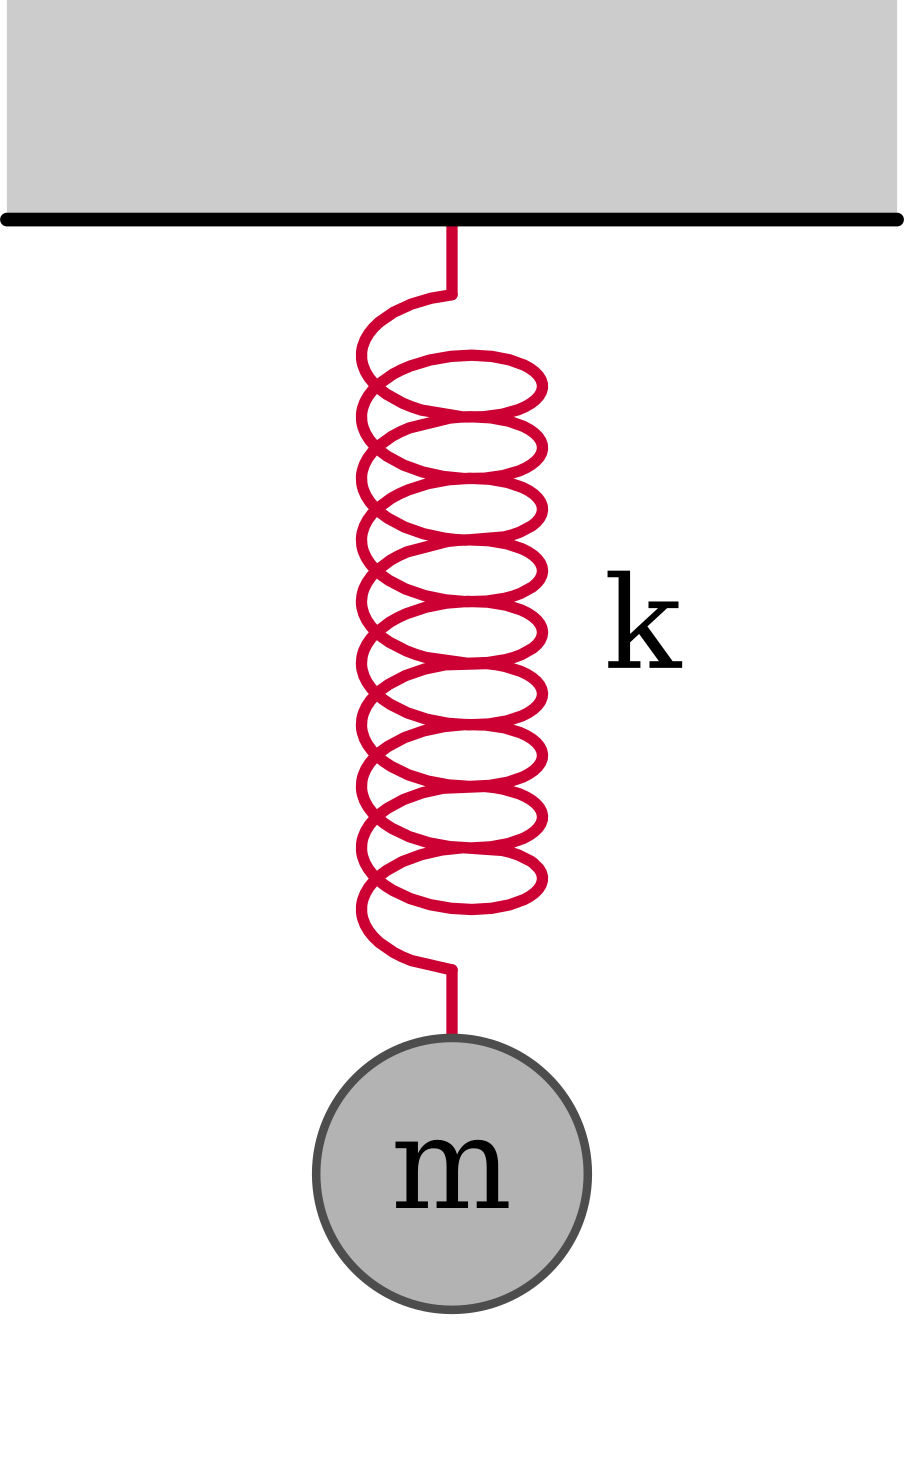
\includegraphics[height=0.3\textheight]{include/vertical_mass_spring}
	\caption{A simple vertical mass-spring system. Taken from \url{{https://commons.wikimedia.org/}}}
	\label{img:vertical_mass_spring}
\end{figure}

When one talks about applying forces to objects, they can probably say that an impulse is delivered. In classical mechanics, impulse is a widely used concept, but for the purposes of this thesis, it is rather important to note how objects respond to impulses. When an impulse is delivered, the object starts to vibrate at all possible frequencies, but having in mind an understanding of resonance frequencies, it is safe to say that not all applied frequencies have equal amplitudes. Thus, some tones in the resulting sound tend to be louder, and others, if not completely silent, highly attenuated. In signal processing, the related concept is called an impulse response and can find some use when discussing digital filters in chapter \ref{chapter:math}. The above-mentioned “chosen” frequencies will be described more in the next section.\\

% TODO: check links to the math chapter

Another essential topic to mention here is why sounds fade in time. This is again connected to the concept of mass-spring systems and the amplitudes of their vibrations. Usually, the bigger these amplitudes are, the louder the resulting sound is, so if the amplitudes didn’t become smaller, we would live in constant unbearable noise. In brief, the fading is caused by the resistance of the medium, in which the sound propagates, and the manner of this propagating. If you imagine air as it was described above --- as many masses connected by invisible springs --- the mechanics of the propagation becomes clear: the sound source pushes the closest mass near it, which due to elasticity pushes its neighbors and returns to its starting location. Then its neighbors, in turn, push their neighbors and return, and so on, until these vibrations come to your ears. The air masses must be pushed again and again for the sound to spread, so it tends to lose its strength along the way, and the further from its source it travels, the smaller the amplitudes of the vibrations become.

\section{Harmonicity and Pitch}

The conversation about how harmonics (or overtones) appear was already started in the previous section. In simple words, not all frequencies of the vibrations caused by delivering an impulse to an object keep their amplitudes for long. The ones that benefit the most from this phenomenon are harmonics, which are the periodic waves with frequencies that are positive integer multiplications of a specific frequency called fundamental, or $f_0$ (Figure \ref{img:harmonics}). For example, if the fundamental frequency is 200\,Hz, the corresponding harmonics are 400\,Hz, 600\,Hz, 800\,Hz, 1\,kHz and so on. Each harmonic can be labeled with a number -- the fundamental frequency one is also called the 1st, and a wave with frequency of 1\,kHz from the example above would be the fifth, or $f_4$.\\

\begin{figure}[h]
	\centering
	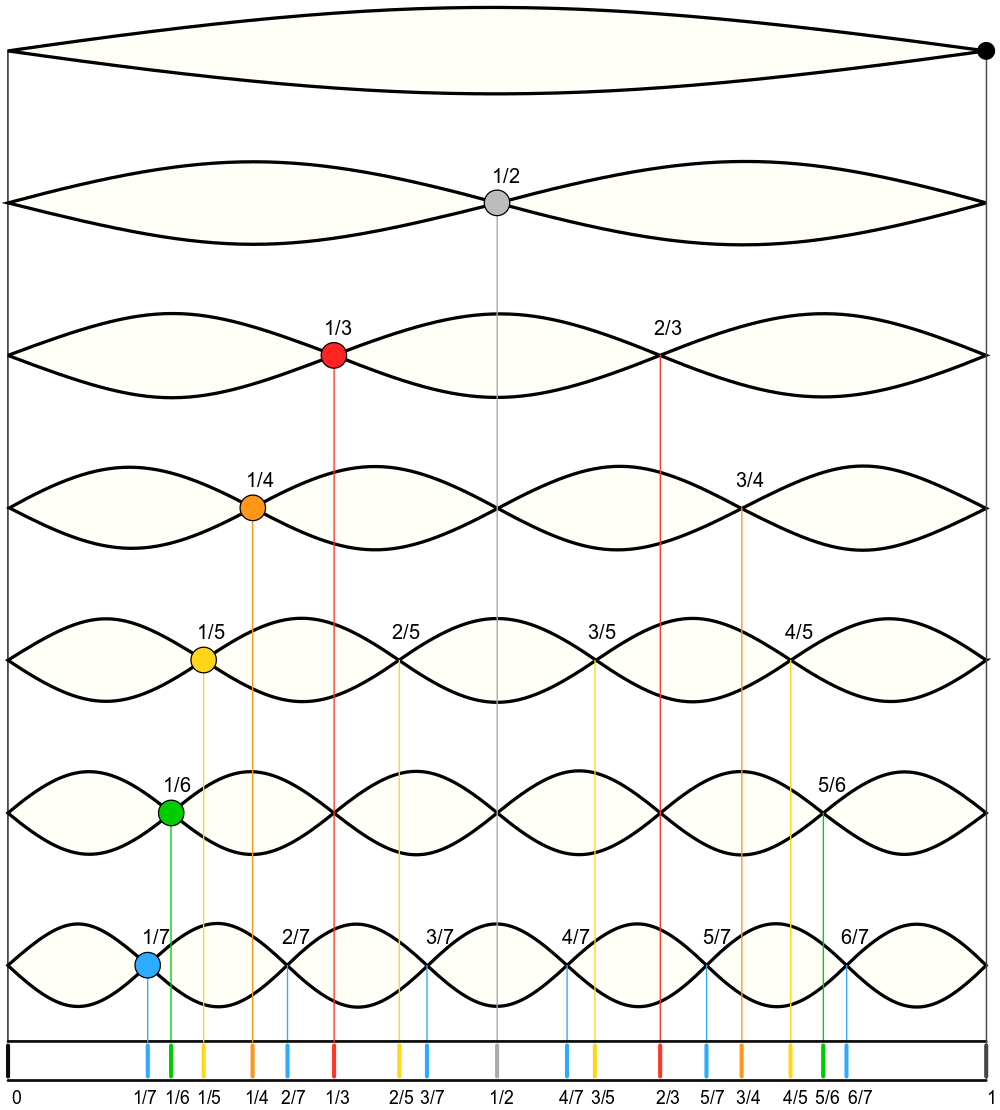
\includegraphics[width=0.6\textwidth]{include/harmonics}
	\caption{First seven harmonics of a sound wave. Taken from \url{{https://commons.wikimedia.org/}}}
	\label{img:harmonics}
\end{figure}

Another explanation of how harmonics appear might be found in [Auditory Neuroscience citation]. When you pluck a guitar string, it doesn't vibrate only as a whole. The same string might be thought of two halves, or three thirds, or even one hundred one hundreds, and that each part of it vibrates separately. So, when the string is plucked, all its harmonics are excited.\\

The most interesting property of harmonics is that they are all periodic at their fundamental frequency. If you sum up any number of adjacent harmonics of a wave, the period of the resulting wave would be equal to the period of the fundamental. This property plays an important role in the perception of pitch.\\





